\begin{figure}[!ht]
\centering
\resizebox{0.6\textwidth}{!}{%
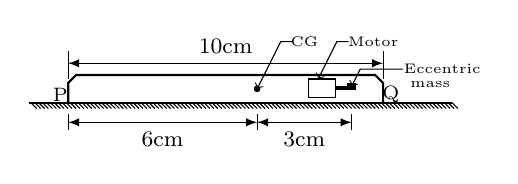
\begin{tikzpicture}
    \draw[black, thick] (-2.5,0) to (2.875,0);
    \draw[black, thick] (-2,0) to (-2,0.25) to (-1.9, 0.35) to (1.9,0.35) to (2.0,0.25) to (2.0,0);
    \foreach \x in {-2.475, -2.425, ..., 2.9} {
        \draw[black, thin] (\x, 0) -- (\x + 0.075, -0.075);
    }
    \draw[black, thin, latex-latex] (-2,0.5) -- (2,0.5) node[midway, above]{\footnotesize 10cm};
    \draw[black, thin] (-2,0.3) to (-2, 0.65);
    \draw[black, thin] (2,0.3) to (2, 0.65);
    \draw[black, thin, latex-latex] (-2, -0.25) -- (0.4,-0.25) node[midway, below]{\footnotesize 6cm};
    \draw[black, thin, latex-latex] (0.4, -0.25) -- (1.6,-0.25) node[midway, below]{\footnotesize 3cm};
    \draw[black, thin] (0.4, -0.35) to (0.4, -0.15);
    \draw[black, thin] (-2, -0.35) to (-2, -0.15);
    \draw[black, thin] (1.6, -0.35) to (1.6, -0.15);
    \filldraw[black] (0.4, 0.175) circle (1pt);
    \draw[black, thin, <-] (0.4, 0.175) to (0.7, 0.775) to (0.85, 0.775);
    \node at (1,0.775) {\tiny CG};
    \filldraw[black] (1.55,0.170) rectangle ++(0.1,0.075);
    \draw[black, very thick] (1.55, 0.185) to ++(-0.15,0);
    \draw[black] (1.4,0.185) to ++(0,0.115) to ++(-0.35,0) to ++(0,-0.24) to ++(0.35,0) to ++(0,0.125);
    \node at (-2.1,0.1){\scriptsize P};
    \node at (2.1,0.1){\scriptsize Q};
    \draw[black, thin, <-] (1.175, 0.3) to (1.4125,0.775) to (1.5625,0.775);
    \node at (1.875, 0.775) {\tiny Motor};
    \draw[black, thin, <-] (1.6,0.2075) to (1.70875,0.425) to (2.25,0.425);
    \node at (2.75,0.425){\tiny Eccentric};
    \node at (2.6, 0.225) {\tiny mass};
    
\end{tikzpicture}
}%

\label{fig:my_label}
\end{figure}